\chapter{RQ4: Fairness and Precision at Realistic Rates}
\label{ch:rq4}
\section{Subgroup error rates}
\todo{Typing speed, keyboard layout, prior experience, gender, etc.\ from the
study's participant attributes (\texttt{students.csv} in the labels manifest).}

\subsection*{Synthetic test students (evaluation harness)}
Simulated people have no demographics, so the harness groups them by terciles
of their simulated habits: typing speed, rhythm variability and build style
(\cref{tab:harness-fairness,fig:harness-fairness}). Honest sessions flagged
range from 0\% (slow typists) to 12\% (steady rhythm) and matched takeovers
detected from 64\% (variable rhythm) to 100\% (slow and steady typists), but
with 10--23 students per group the intervals overlap. The variable-rhythm
group is the one to watch on real data: a typist whose own timing is
noisy gives the per-pair baseline wide spreads, so a different typist stands
out less. The machinery is in place; what it shows is that a
test set of 36 cannot establish or rule out a disparity of this size, which
argues for pooling subgroup analysis across all study phases or recruiting
towards the top of the planned 60--80.

% Generated by studentide.harness (synthetic:synth-v1-n120-s2026-b8-m30, test split, 36 students). Do not edit by hand.
\begin{table}[ht]
  \centering\small
  \caption{RQ4: error rates by subgroup for the thesis detector on the synthetic test students (95\% student-bootstrap intervals). Synthetic subgroups are terciles of the simulated habit profile; the study replaces them with recorded attributes.}
  \label{tab:harness-fairness}
  \resizebox{\linewidth}{!}{\begin{tabular}{@{}llrccc@{}}
    \toprule
    Attribute & Group & Students & Honest flagged & FA/h & Takeover detected \\
    \midrule
    build\_style & outline-first & 23 & 9\% {\scriptsize[2, 17]} & 0.39 {\scriptsize[0.04, 0.91]} & 61\% {\scriptsize[43, 78]} \\
     & top-down & 13 & 4\% {\scriptsize[0, 12]} & 0.08 {\scriptsize[0.00, 0.23]} & 69\% {\scriptsize[46, 92]} \\
    rhythm & medium & 12 & 8\% {\scriptsize[0, 21]} & 0.17 {\scriptsize[0.00, 0.42]} & 75\% {\scriptsize[50, 100]} \\
     & steady & 13 & 8\% {\scriptsize[0, 19]} & 0.54 {\scriptsize[0.00, 1.46]} & 54\% {\scriptsize[31, 85]} \\
     & variable & 11 & 5\% {\scriptsize[0, 14]} & 0.09 {\scriptsize[0.00, 0.27]} & 64\% {\scriptsize[36, 91]} \\
    typing\_speed & fast & 12 & 4\% {\scriptsize[0, 12]} & 0.17 {\scriptsize[0.00, 0.50]} & 75\% {\scriptsize[50, 100]} \\
     & medium & 14 & 14\% {\scriptsize[4, 29]} & 0.57 {\scriptsize[0.07, 1.42]} & 43\% {\scriptsize[21, 71]} \\
     & slow & 10 & 0\% {\scriptsize[0, 0]} & 0.00 {\scriptsize[0.00, 0.00]} & 80\% {\scriptsize[60, 100]} \\
    \bottomrule
  \end{tabular}}
\end{table}


\begin{figure}[ht]
  \centering
  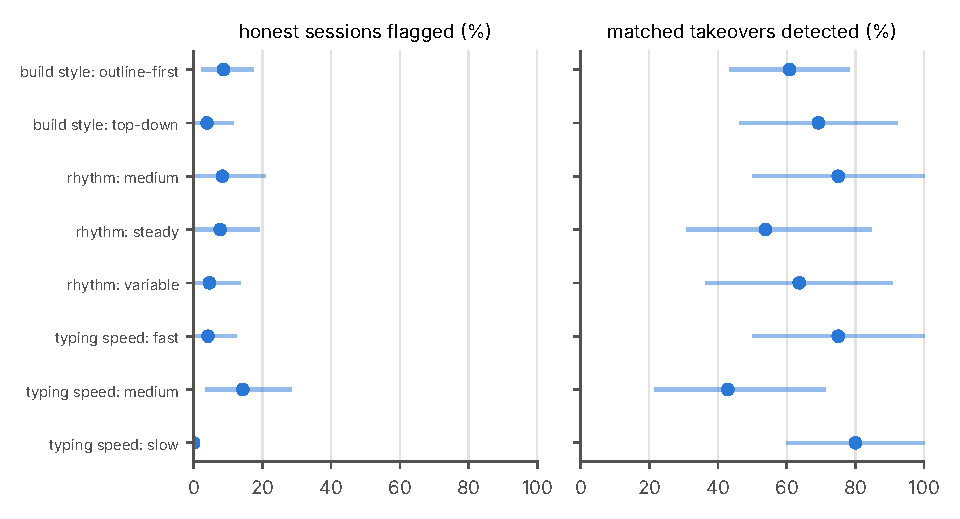
\includegraphics[width=\linewidth]{harness-fairness}
  \caption{Error rates by synthetic subgroup, 95\% student-bootstrap intervals.}
  \label{fig:harness-fairness}
\end{figure}

\section{Precision at low prevalence}
Precision $= \frac{\mathrm{TPR}\,\pi}{\mathrm{TPR}\,\pi + \mathrm{FPR}(1-\pi)}$
at $\pi = 1/100$ and $1/500$.

On the synthetic test students the thesis detector finds 92\% of non-honest
sessions and flags 7\% of honest ones (\cref{tab:harness-precision}). If 1 in 100
sessions involved a switch, about 12\% of flagged sessions would be real (95\%
interval 7--26\%); at 1 in 500, about 3\%. Put the other way, a teacher would
see 7.5 honest sessions flagged for every real one at 1 in 100, and 38 at 1 in
500. The key-pair channel raised detection but not the honest flag rate, so
precision barely moved (11\% before). The baselines, with lower TPR and similar
or higher FPR, are worse (4--6\% at 1 in 100). Lowering the operating point
helps but cannot fix this (\cref{fig:harness-precision}): at the lowest
calibrated false-alarm rate (3\% of honest sessions flagged, 81\% of
non-honest ones caught) precision at 1 in 100 reaches about 23\%.

This is the quantitative case for the design rule that a flag only ever starts
a conversation: at realistic rates most flags will be honest students, and any
use of the tool as evidence of misconduct would be wrong most of the time.

% Generated by studentide.harness (synthetic:synth-v1-n120-s2026-b8-m30, test split, 36 students). Do not edit by hand.
\begin{table}[ht]
  \centering\small
  \caption{RQ4: what a flag means at realistic cheating rates (synthetic test students, operating point of \cref{tab:harness-methods}). TPR: non-honest sessions with an alarm after the switch; FPR: honest sessions with any alarm. Precision $= \mathrm{TPR}\,\pi / (\mathrm{TPR}\,\pi + \mathrm{FPR}(1-\pi))$; honest flags per real one = $\mathrm{FPR}(1-\pi)/(\mathrm{TPR}\,\pi)$.}
  \label{tab:harness-precision}
  \resizebox{\linewidth}{!}{\begin{tabular}{@{}lccccrr@{}}
    \toprule
    Method & TPR & FPR & Prec.\ $\pi=1/100$ & Prec.\ $\pi=1/500$ & Honest per real (1/100) & (1/500) \\
    \midrule
    Two-channel CUSUM & 83\% & 7\% {\scriptsize[1, 12]} & 10.7\% {\scriptsize[6, 38]} & 2.3\% {\scriptsize[1, 11]} & 8.3 & 41.9 \\
    Scaled Manhattan & 53\% & 12\% & 4.1\% & 0.8\% & 23.2 & 117.0 \\
    TypeNet-style LSTM & 39\% & 10\% & 3.9\% & 0.8\% & 24.4 & 123.0 \\
    Nosi-style L-scale & 47\% & 7\% & 6.4\% & 1.3\% & 14.7 & 74.3 \\
    \bottomrule
  \end{tabular}}
\end{table}


\begin{figure}[ht]
  \centering
  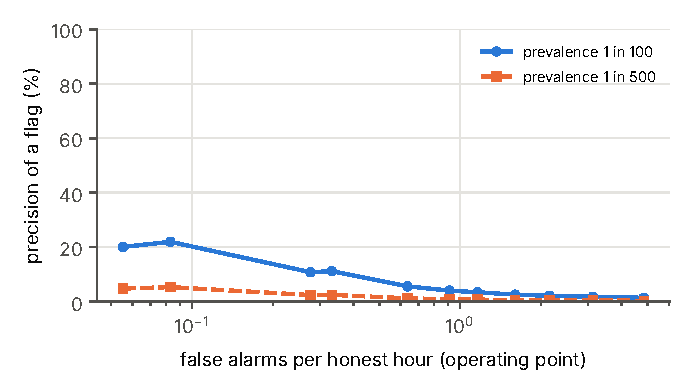
\includegraphics[width=0.65\linewidth]{harness-precision}
  \caption{Precision of a flag by operating point at two prevalences (thesis
    detector, synthetic test students).}
  \label{fig:harness-precision}
\end{figure}

\section{Summary}
